\section{Autocompare with OpenACC}

The PCAST OpenACC autocompare feature works by executing each OpenACC compute kernel on both the GPU and the host CPU.
This keeps the values in system memory in sync with the values in GPU device memory, assuming the same computation is done correctly on each. Figure 1 illustrates the flow of regular OpenACC program with and without turning on the PCAST autocompare option. The computationally intensive part of the illustration can consist of more than one single kernel.

\begin{figure*}[t]
    \centering
    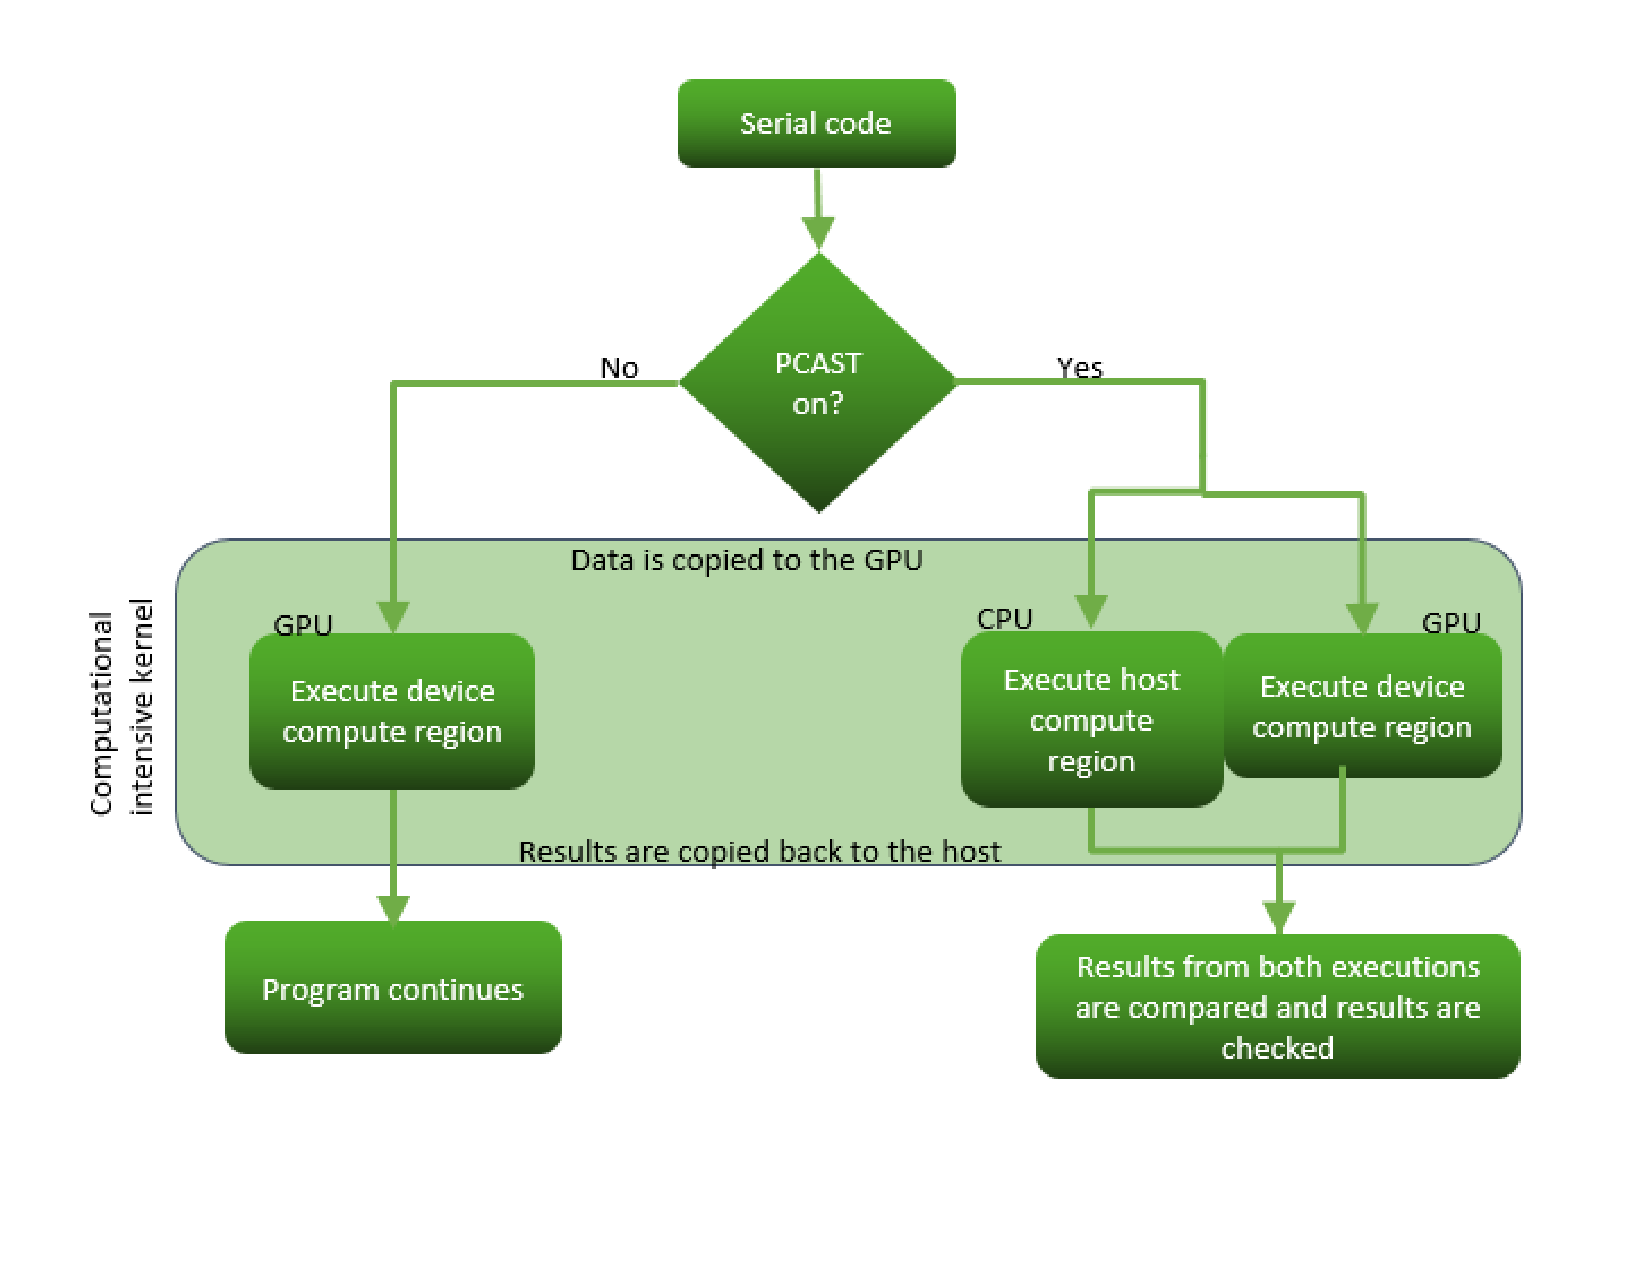
\includegraphics [width=1\linewidth] {flow_chart.pdf}
    \caption{An overview of the autocompare functionality.}
    \label{fig:cfg_figure}
\end{figure*}


The next, equally important step is to compare the computed values on the CPU with those on the GPU.
We assume that the CPU values are the reference values, and the GPU values are the ones being tested.
Ideally, we would compare only the data that was changed in a compute construct.
In small sample programs, this is easy to automatically determine, but in general this is not feasible.
Instead, we studied several options for choosing what values to compare between host and device, and at what point to do the compare.
\begin{enumerate}
\item The runtime could compare all the data in GPU memory to the corresponding CPU memory after each kernel launch.
This is feasible, but likely to be prohibitively expensive.
Large applications can fill the 16GB device memory (on an NVIDIA Pascal GPU), and bringing that much data back and comparing it after each kernel launch would be very expensive.
However, it would certainly be able to identify the specific kernel where results start to diverge.

\item The runtime could compare data only at the end of a compute construct, and only data that is either in an explicit data clause or is explicitly referenced in the construct.
This is less costly than comparing all data, but it could miss updated global data that is modified only in routines called from the compute construct.

\item The runtime could compare data only at the end of a compute construct, and only that data in an explicit data clause on that compute construct (not data implicitly copied to the GPU, or in a clause for an outer data construct).
This is even less costly, and only compares data that the programmer thought important enough to include in a data clause.

\item The runtime could compare data only at the end of a data region, and only the data in explicit data clauses.
This is likely to be less costly because a data region typically contains many compute constructs, such as an outer loop that contains a compute construct.
However it is less precise about identifying which particular compute construct caused the divergence.

\item The runtime could compare data when it would otherwise be copied back to the host.
This would be at the end of a compute or data construct, or at an OpenACC \emph{update} directive.
Since the data is already being copied to the host, the only overhead is the actual compare.
This method would be even less precise about identifying where the divergent computations occurred.

\item Finally, the runtime could leave the choice to the user.
This would allow the user to insert a runtime call or a directive that tells the runtime when to compare data, and what data to compare.
We considered two options: one where the user chose one or more variables or arrays to compare, and a second where the user asks the runtime to compare all variables and arrays present in device memory to the corresponding host memory locations.
\end{enumerate}

In all cases, since the same computations are done on the CPU as well as the GPU, the OpenACC runtime must allow for this and not do any actual data downloads from the device memory to host memory.
This means \emph{update host} directives and \emph{copyout} actions from data directives should not update the host values.

There are errors that the PCAST OpenACC autocompare feature can not detect.
In particular, since the compare point requires synchronization with the device, any errors due to misplaced or erroneous \emph{async} clauses, or missing \emph{wait} directives or clauses may be hidden.
Also, OpenACC has features that allow different computations on the host as on the device, to allow for different algorithmic formulations that are more appropriate for each processor.
Such a feature can allow for programming mistakes that are hard to detect.
Again, the goal is to detect numeric computational differences between two executions, not to find all errors.
